\subsection{EXPORTAÇÃO DE GRADES HORÁRIAS}

Considerando a necessidade de exportar as grades horárias para fora do sistema, e a sua natureza tabular, implementou-se a funcionalidade de \textit{download} das grades como planilhas Excel, no formato XLSX.

Para possibilitar a exportação neste formato, utilizou-se o pacote \textit{Node ExcelJs}, que providencia a classe ``WorkBook'', a qual facilita a construção de arquivos de planilhas Excel utilizando a linguagem \textit{JavaScript}. O resultado final desta implementação pode ser visto na \autoref{fig:gradeExportada}.

\begin{figure}[!htb]
	\centering
	\caption{Grade horária exportada para planilha}
	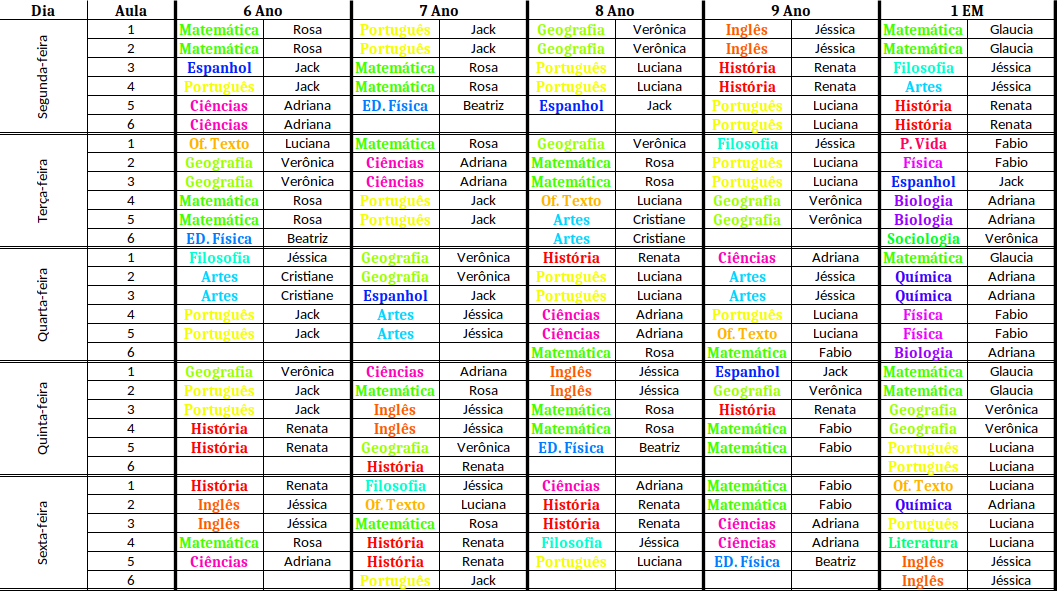
\includegraphics[width=1\textwidth]{./dados/figuras/gradeExportada}
	\fonte{Autor}
	\label{fig:gradeExportada}
\end{figure}

Para possibilitar a realização do \textit{download} das grades horárias, acrescentou-se um botão à interface. Adicionalmente, foram adicionados botões para navegar entre as diferentes grades geradas, e exibir mais informações sobre a grade selecionada.